\documentclass[english,11pt]{beamer}

\DeclareMathOperator{\Cov}{Cov}
\DeclareMathOperator{\Var}{Var}
\DeclareMathOperator{\E}{\mathbb{E}}
\DeclareMathOperator{\Proba}{\mathbb{P}}

\newcommand{\Covb}[2]{\ensuremath{\Cov\!\left[#1,#2\right]}}
\newcommand{\Eb}[1]{\ensuremath{\E\!\left[#1\right]}}
\newcommand{\Pb}[1]{\ensuremath{\Proba\!\left[#1\right]}}
\newcommand{\Varb}[1]{\ensuremath{\Var\!\left[#1\right]}}

% norm
\newcommand{\norm}[1]{\| #1 \|}

\newcommand{\indep}{\rotatebox[origin=c]{90}{$\models$}}





\usepackage{mathptmx,amsmath,amssymb,graphicx,bibentry,bbm,babel,ragged2e}

\makeatletter

\newcommand{\noun}[1]{\textsc{#1}}
\newcommand{\jitem}[1]{\item \begin{justify} #1 \end{justify} \vfill{}}
\newcommand{\sframe}[2]{\frame{\frametitle{#1} #2}}

\newenvironment{centercolumns}{\begin{columns}[c]}{\end{columns}}
%\newenvironment{jitem}{\begin{justify}\begin{itemize}}{\end{itemize}\end{justify}}









%\usetheme{Warsaw}
%\setbeamertemplate{footline}[text line]{}
%\setbeamercolor{structure}{fg=purple!50!blue, bg=purple!50!blue}
%\setbeamersize{text margin left=15pt,text margin right=15pt}




\usetheme{Boadilla}


% cybergeo palette (from Clem server)
% #1C6F91, "#df691a", "#77c5ba", "orange", "#2db92d", "#e1ff2f", "#ff2313", "#bbab61
% redefine palette
\definecolor{cybblue}{HTML}{1C6F91}
\definecolor{cyborange}{HTML}{DF691A}
\definecolor{cybbluegreen}{HTML}{77C5BA}
\definecolor{cybgreen}{HTML}{2DB92D}
\definecolor{cybgreenyellow}{HTML}{E1FF2F}
\definecolor{cybred}{HTML}{FF2313}
\definecolor{cybglaucous}{HTML}{BBAB61}


\setbeamercolor{structure}{fg=cybblue}
%\setbeamercolor{footline}{fg=orange, bg=orange}

\setbeamercovered{transparent}


\addtobeamertemplate{title page}{%\hspace{-0.4cm}
\vspace{-0.8cm}
\hspace{-0.5cm}
%\includegraphics[height=1.2cm,width=1.2\textwidth]{template/bandeau3}\\
}{%
%\begin{textblock*}{150mm}(-1cm,-1.5cm)
%\end{textblock*}
}


\setbeamertemplate{footline}{
\hspace{0.2cm}

\includegraphics[height=1cm]{template/medium}
\hfill

\includegraphics[height=1cm]{template/eu}
\hspace{0.2cm}
\vspace{0.2cm}
}





\@ifundefined{showcaptionsetup}{}{%
 \PassOptionsToPackage{caption=false}{subfig}}
\usepackage{subfig}

\usepackage[utf8]{inputenc}
\usepackage[T1]{fontenc}


\usepackage[usenames,dvipsnames]{pstricks}
\usepackage{epsfig}



\makeatother

\begin{document}


\title{Towards a Theory of Co-evolutive Networked Territorial Systems: Insights from Transportation Governance Modeling in Pearl River Delta, China}

\author{J.~Raimbault$^{1,2}$\\
\texttt{juste.raimbault@polytechnique.edu}
}


\institute{$^{1}$UMR CNRS 8504 G{\'e}ographie-cit{\'e}s\\
$^{2}$UMR-T IFSTTAR 9403 LVMT\\
}


\date{Medium Project Seminar\\\smallskip
4th December 2016
}


{


\setbeamertemplate{footline}{
\hspace{0.2cm}

\includegraphics[height=1cm]{template/medium}
\hfill
\large This Project is funded by the European Union

\includegraphics[height=1cm]{template/eu}
\hspace{0.2cm}
\vspace{0.2cm}
}


\frame{\maketitle}

}




%%%%%%%%%%%%%%%%%%%
%% ABSTRACT

%Recent advances in Theoretical and Quantitative Geography have witnessed the co-construction of geographical theories, complex models of simulation and Empirical analysis. We build on this legacy to shed light on relations between territories and networks. Our contribution consists in two distincts parts. First we develop a new theory of territorial systems, that emphasizes on the role of networks in co-evolutive processes. More precisely, we speculate, building on several modeling and empirical previous contributions, that within Pumain’s Evolutive Urban Theory [Pumain, 1997], the existence of co-evolutive subsystems is equivalent to the existence of morphogenetic processes in which networks are significant drivers. Implications include the necessity of networks in explaining territorial systems dynamics, but also a modular decomposition of these systems into local stationary processes in space or time.
%In a second part, we discuss practical implications of the theory through the adaptation of a agent- based model introduced in [Le Néchet and Raimbault, 2015], which simulates the co-evolution of land-use and transportation infrastructure within a Mega-city Region. In particular, it includes game theoretical modeling of decision making processes for transportation governance. The model is partially validated on synthetic data by retrieving expected stylized facts on emergent infrastructure. We propose then to apply it to the Mega-city Region of Pearl River Delta, China, which is very typical of included characteristics such as the presence of a strong competition between inner cities and the recent realization, construction or planning of numerous large-scale transportation infrastructures. Calibration of the model will allow first to infer information on potentially hidden governance processes when applied on real or planned infrastructure, and secondly to compare among different possible governance frameworks when applied on hypothetical optimized infrastructure.






%%%%%%%%%%%%%%%%%%%
\section{Introduction}
%%%%%%%%%%%%%%%%%%%


\sframe{Complex Urban Systems}{

\centering

%\includegraphics[width=0.45\textwidth,height=0.6\textheight]{}
\hspace{0.1cm}
%\includegraphics[width=0.45\textwidth,height=0.6\textheight]{}

{\tiny Source : Wikipedia}

}



\sframe{Complex Systems Approaches in Science}{

% exemples of CS Approaches / emergence 
% -> why CS ?

$\rightarrow$ Failure of reductionism already highlighted by Anderson in 1972~\cite{anderson1972more}


$\rightarrow$


}


\sframe{Theoretical and Quantitative Geography}{

% adapt Sander's schema (adding methods and tools)
%  Q : each "space" is indeed a dimension , and links are rotations ? not euclidian space.

\textit{Extended framework for TQG~\cite{livet2010}}

\bigskip
\bigskip

\centering

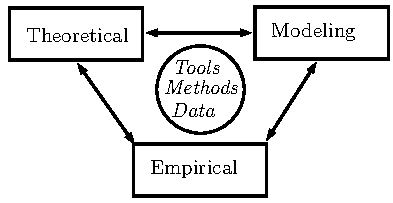
\includegraphics[height=0.5\textheight,width=0.8\textwidth]{figures/tqg.pdf}

}


%%%%%%%%%%%%%%%%%%%
\section{Towards a Theory}
%%%%%%%%%%%%%%%%%%%


\sframe{Meso-scale Coupled Growth}{

}



\sframe{Meso-scale Urban Growth}{

}


\sframe{Coupled Growth and Correlations}{

}


\sframe{Macro-scale Growth and Network Necessity}{

}



%%%%%%%%%%%%%%%%%%%%%%%%%%%%
\sframe{Theory : Pillars}{
\begin{enumerate}
\item \textit{Networked Human Territories} $\rightarrow$ Raffestin approach to territory combined with Dupuy theory of networks.
\item \textit{Evolutive Urban Theory} $\rightarrow$ City Systems as complex Adaptive systems, applied to human settlements in general and thus territorial systems.
\item \textit{Urban Morphogenesis} $\rightarrow$ Morphogenesis as autonomous rules to explain growth of urban form. Used as the provider of modular decompositions.
\item \textit{Boundaries and Co-evolution} $\rightarrow$ Co-evolution as the existence of \textit{niche}, consequence of boundary patterns.
\end{enumerate}
}
%%%%%%%%%%%%%%%%%%%%%%%%%%%%



%%%%%%%%%%%%%%%%%%%%%%%%%%%%
\sframe{Theory : Specification}{
\begin{itemize}
\jitem{Previous def. of territorial systems}
\jitem{Modular decomposition and stationarity : existence of scales}
\jitem{Feedback loops between and inside scales yield weak emergence, thus complexity}
\jitem{Morphogenesis gives modular decomposition and co-evolution}
\jitem{\textbf{Main assumption.} Necessity of Networks : networks are necessary component of co-evolutive niches.}
\end{itemize}
}
%%%%%%%%%%%%%%%%%%%%%%%%%%%%







%%%%%%%%%%%%%%%%%%%
\section{Transportation Governance}
%%%%%%%%%%%%%%%%%%%










\sframe{Conclusion}{


\bigskip
\bigskip
\bigskip


\footnotesize{ - All code and data available at \texttt{https://github.com/JusteRaimbault/CityNetwork/tree/master/Models\\
/Governance}

}

}




\sframe{Reserve slides}{

\centering

\Large

\textbf{Reserve Slides}

}




%%%%%%%%%%%%%%%%%%%%%
\begin{frame}[allowframebreaks]
\frametitle{References}
\bibliographystyle{apalike}
\bibliography{/Users/Juste/Documents/ComplexSystems/CityNetwork/Biblio/Bibtex/CityNetwork,biblio}
\end{frame}
%%%%%%%%%%%%%%%%%%%%%%%%%%%%




\sframe{Reserve slides}{


}









\end{document}







